%%%%%%%%%%%%%%%%%%%%%%%%%%%%%%%%%%%%%%%%%
% Thin Sectioned Essay
% LaTeX Template
% Version 1.0 (3/8/13)
%
% This template is based on a downloaded from:
% http://www.LaTeXTemplates.com
%
% Original Author:
% Nicolas Diaz (nsdiaz@uc.cl) with extensive modifications by:
% Vel (vel@latextemplates.com)
% and adjustments by 
% Thuy Tran 
%
% License:
% CC BY-NC-SA 3.0 (http://creativecommons.org/licenses/by-nc-sa/3.0/)
%
%%%%%%%%%%%%%%%%%%%%%%%%%%%%%%%%%%%%%%%%%

%----------------------------------------------------------------------------------------
%	PACKAGES AND OTHER DOCUMENT CONFIGURATIONS
%----------------------------------------------------------------------------------------

\documentclass[a4paper, 12pt]{report} % Font size (can be 10pt, 11pt or 12pt) and paper size (remove a4paper for US letter paper)

\usepackage[protrusion=true,expansion=true]{microtype} % Better typography
\usepackage{graphicx} % Required for including pictures
\usepackage{wrapfig} % Allows in-line images

\usepackage{mathpazo} % Use the Palatino font
\usepackage[T1]{fontenc} % Required for accented characters
\usepackage[utf8]{inputenc} 
\usepackage[ngerman]{babel}
\linespread{1.05} % Change line spacing here, Palatino benefits from a slight increase by default

\makeatletter
\renewcommand\@biblabel[1]{\textbf{#1.}} % Change the square brackets for each bibliography item from '[1]' to '1.'
\renewcommand{\@listI}{\itemsep=0pt} % Reduce the space between items in the itemize and enumerate environments and the bibliography

\renewcommand{\maketitle}{ % Customize the title - do not edit title and author name here, see the TITLE block below
\begin{flushright} % Right align
{\LARGE\@title} % Increase the font size of the title

\vspace{50pt} % Some vertical space between the title and author name

{\large\@author} % Author name
\\\@date % Date

\vspace{40pt} % Some vertical space between the author block and abstract
\end{flushright}
}

%----------------------------------------------------------------------------------------
%	TITLE
%----------------------------------------------------------------------------------------

\title{\textbf{}\\ % Title
Terminal zur Bearbeitung von ARX-Daten mit R} % Subtitle

\author{\textsc{Alexander Beischl und Thuy Tran} % Author
\\{\textit{Technische Universität München}}} % Institution

\date{\today} % Date

%----------------------------------------------------------------------------------------

\begin{document}

\maketitle % Print the title section

%----------------------------------------------------------------------------------------
%	ABSTRACT AND KEYWORDS
%----------------------------------------------------------------------------------------

\renewcommand{\abstractname}{Zusammenfassung} % Uncomment to change the name of the abstract to something else

\begin{abstract}
Morbi tempor congue porta. Proin semper, leo vitae faucibus dictum, metus mauris lacinia lorem, ac congue leo felis eu turpis. Sed nec nunc pellentesque, gravida eros at, porttitor ipsum. Praesent consequat urna a lacus lobortis ultrices eget ac metus. In tempus hendrerit rhoncus. Mauris dignissim turpis id sollicitudin lacinia. Praesent libero tellus, fringilla nec ullamcorper at, ultrices id nulla. Phasellus placerat a tellus a malesuada.
\end{abstract}


\vspace{30pt} % Some vertical space between the abstract and first section
%----------------------------------------------------------------------------------------

\tableofcontents


%----------------------------------------------------------------------------------------
%	ESSAY BODY
%----------------------------------------------------------------------------------------

\chapter{Einführung}\label{einführung}

This statement requires citation \cite{latexcompanion}; this one does too \cite{einstein}. Lorem ipsum dolor sit amet, consectetur adipiscing elit. Aenean dictum lacus sem, ut varius ante dignissim ac. Sed a mi quis lectus feugiat aliquam. Nunc sed vulputate velit. Sed commodo metus vel felis semper, quis rutrum odio vulputate. Donec a elit porttitor, facilisis nisl sit amet, dignissim arcu. Vivamus accumsan pellentesque nulla at euismod. Duis porta rutrum sem, eu facilisis mi varius sed. Suspendisse potenti. Mauris rhoncus neque nisi, ut laoreet augue pretium luctus. Vestibulum sit amet luctus sem, luctus ultrices leo. Aenean vitae sem leo.

Nullam semper quam at ante convallis posuere. Ut faucibus tellus ac massa luctus consectetur. Nulla pellentesque tortor et aliquam vehicula. Maecenas imperdiet euismod enim ut pharetra. Suspendisse pulvinar sapien vitae placerat pellentesque. Nulla facilisi. Aenean vitae nunc venenatis, vehicula neque in, congue ligula.

%------------------------------------------------

\section*{R}\label{r}
R ist eine Programmiersprache und Entwicklungsumgebung, die für statistische Berechnungen und Graphen unter John Chambers von Bell Laboratories entwickelt wurde. Sie ist ein GNU-Projekt, bei dem die Entwicklung von freier Software im Mittelpunkt steht. R weist große Ähnlichkeiten zu der Programmiersprache S auf, ein weiteres GNU-Projekt, welches weitgehend auch unter R läuft. \cite{rproject}

R bietet standardmäßig alle Hauptfunktionen an für die statistische Analyse von Datensätzen an und ist einfach zu erweitern, weswegen es vor allem für wissenschaftliche Arbeiten verwendet wird. Es ist mit R einfach, statistische Funktionen auf große Datenmengen anzuwenden.  


%------------------------------------------------

\section*{ARX}
ARX ist eine freie Software zur Anonymisierung von medizinischen Datensätzen, die von Fabian Prasser und Florian Kohlmayer vom Institut für medizinische Statistik und Epidemiologie an der Technischen Universität München entwickelt wurde.



\chapter{Anwenderdokumentation}
\section{Übersicht}
Das R-Terminal dient dazu, über eine externe Schnittstelle R aufzurufen und zu bedienen. Dies soll vor allem dazu genutzt werden, um Tabellen aus ARX einzuladen und Skripte auszuführen, und gleichzeitig die im Kapitel \ref{einführung} beschriebenen Probleme zu umgehen. Das R-Terminal ist kompatibel mit Windows, der Linux Distribution Ubuntu und OS X, von denen jeweils die folgenden Versionen im Rahmen der Entwicklung getestet wurden: 

\begin{itemize}
\item Windows 10 Education (Version 1511)
\item OS X El Capitan (Version 10.11.1)
\item macOS Sierra (Version 10.12.2)
\item Ubuntu
\end{itemize}

%insert screenshot for linux and the correct ubuntu/opensuse version

In den folgenden Abschnitten werden die Grundfunktionen und zusätzliche Features des R-Terminals beschrieben. 
\section{}

\begin{figure}[htpb]
\centering
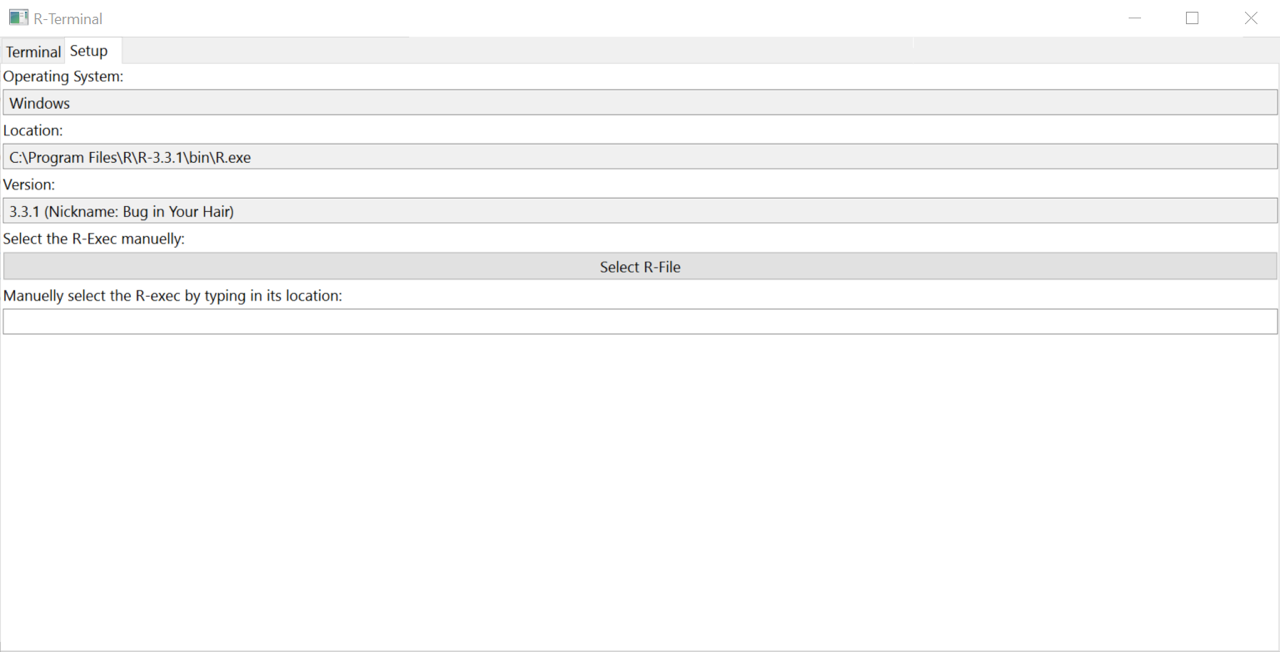
\includegraphics[width=0.8\textwidth]{R-TerminalWindows}
\caption{R-Terminal: \textit{Terminal} unter Windows 10 Education (Version 1511)}
\label{rterminalwindows}
\end{figure}

\begin{figure}[htpb]
\centering
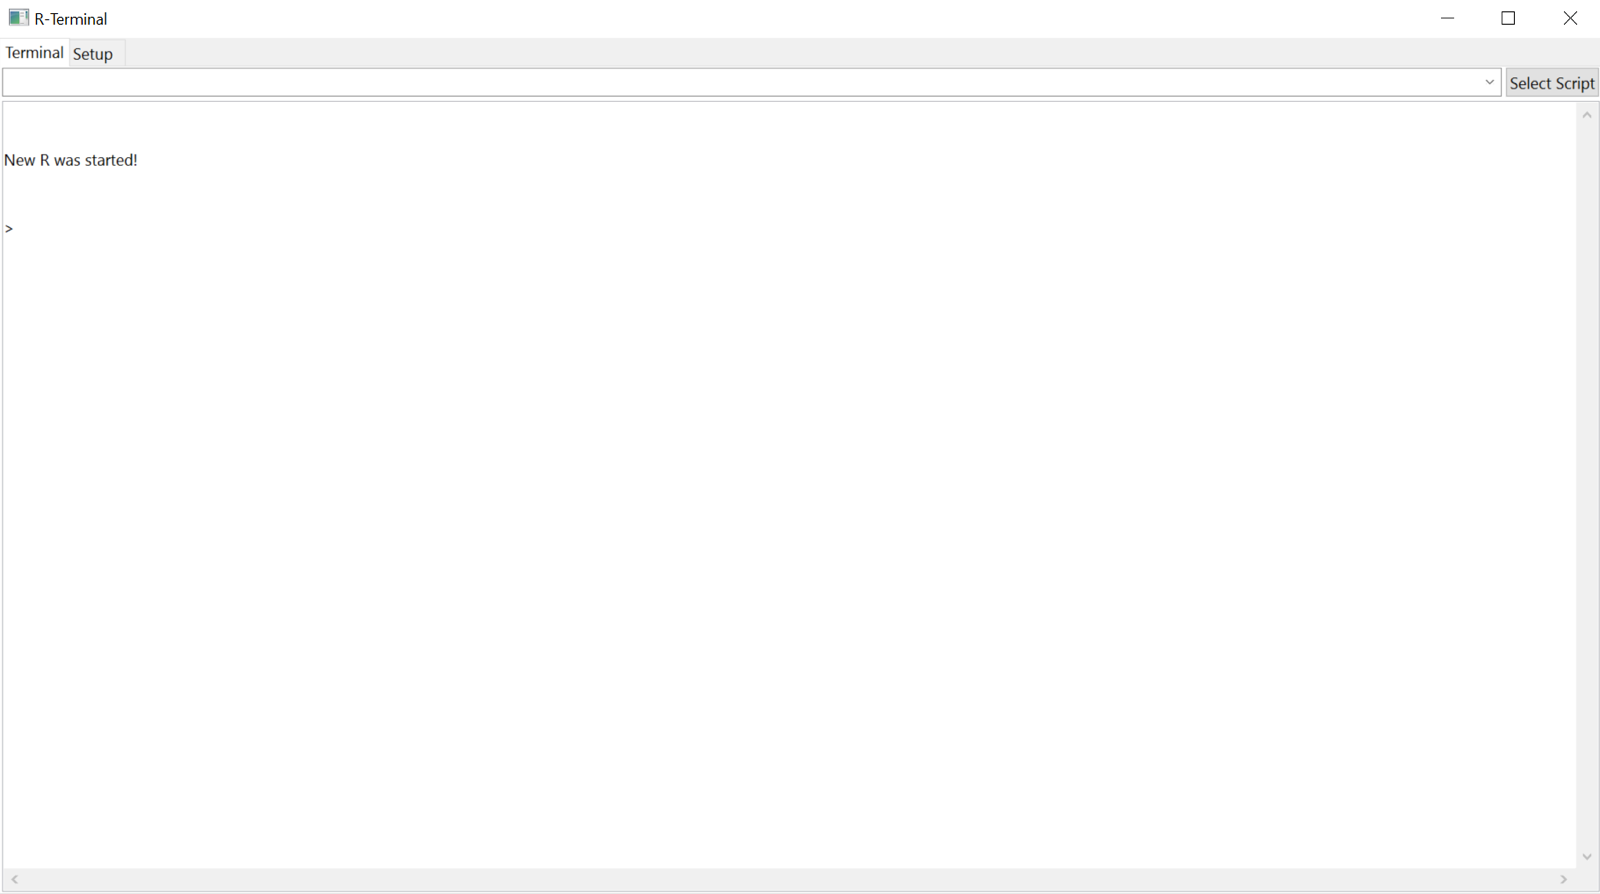
\includegraphics[width=0.8\textwidth]{rterminalwindows}
\caption{R-Terminal: \textit{Setup} unter Windows 10 Education (Version 1511)}
\label{rterminalwindows}
\end{figure}

\begin{figure}[htpb]
\centering
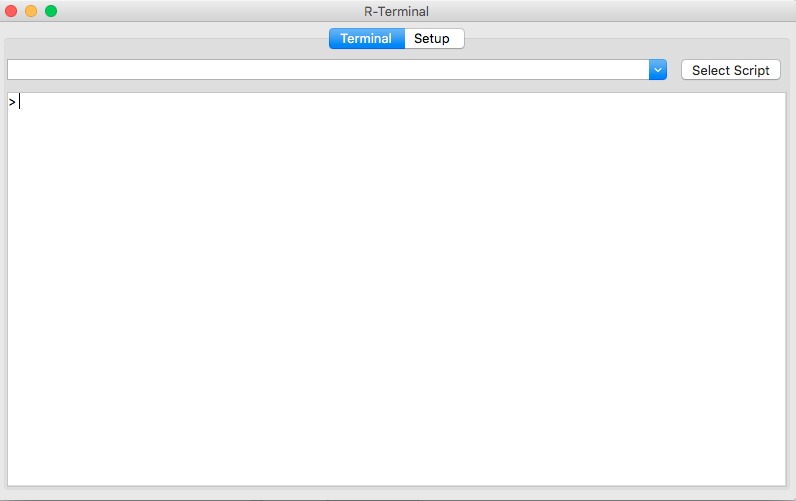
\includegraphics[width=0.8\textwidth]{R-Terminal}
\caption{R-Terminal: \textit{Terminal} unter OS X (Version 10.11.1)}
\label{rterminalmac}
\end{figure}

\begin{figure}[htpb]
\centering
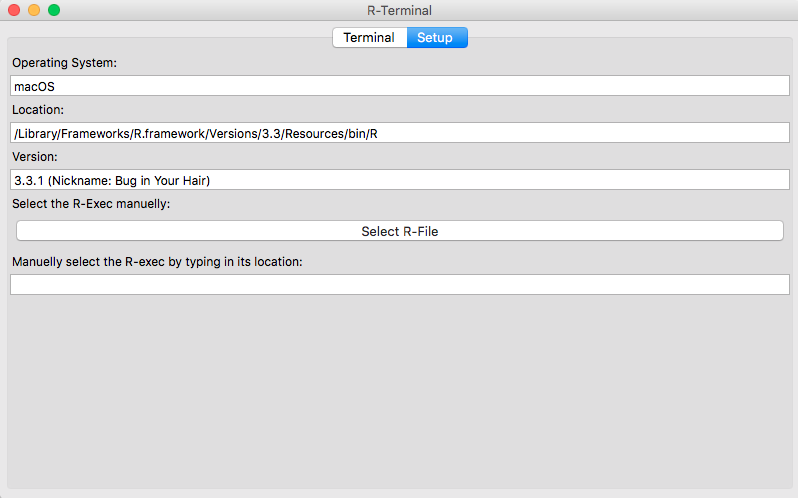
\includegraphics[width=0.8\textwidth]{rterminalsetup}
\caption{R-Terminal: \textit{Setup} unter OS X (Version 10.11.1)}
\label{macsetup}
\end{figure}

In Abbildung \ref{rterminalmac} ist das R-Terminal unter OS X (hier Version 10.11.1) zu sehen. Das Terminal verfügt über die beiden Tabs \textit{Terminal} und \textit{Setup} (s. \ref{macsetup)}. Unter \textit{Setup} wird entweder eine R-Version auf dem Rechner gesucht und automatisch ausgeführt oder es wird vom Benutzer selber der Pfad zu der gewünschten R-Version angegeben.

\newpage

\chapter{Entwicklerdokumentation}

\section{Verwendete Technologien}

Das \textit{R-Terminal} wurde mit der Entwicklungsumgebung \textit{Eclipse} entwickelt.
Als Programmiersprache wurde \textit{Java} gewählt. Zur Realisierung der graphischen Benutzeroberfläche wurde \textit{SWT} gewählt, genauere Details hierzu werden in \ref{swt} erläutert.



\section{Architektur des R-Terminals}

Die Software des \textit{R-Terminal} ist in zwei Komponenten aufgeteilt, welche als getrennte "`Packages"' vorliegen. Das erste Package beinhaltet die graphische Benutzeroberfläche, das Zweite beinhaltet die gesamte Integration von \textit{R} in \textit{Java}, es stellt also alle Funktionen zur Verfügung und verwaltet die Kommunikation zwischen \textit{R} und dem \textit{Java}-Programm.

Durch die Trennung von graphischer Benutzeroberfläche und der \textit{R}-Integration können alle Funktionen auch ohne die GUI ausgeführt und verwendet werden.

\section{Graphische Benutzeroberfläche}\label{gui}

\begin{samepage}

Das erste Package, benannt "`org.deidentifier.arx.gui"', erzeugt und verwaltet die graphische Benutzeroberfläche. Es umfasst sieben Klassen:
\begin{itemize}
	\item RMain
	\item RTerminal
	\item RSetupTab
	\item RTerminalTab
	\item RBrowserWindow
	\item RLayout
	\item RCommandListener
\end{itemize}
\end{samepage}

\subsection{RMain}

Um das Programm mit der graphischen Benutzeroberfläche zu starten, muss die Methode "`main"' der Klasse \textit{RMain} aufgerufen werden. Diese erzeugt ein neues Display sowie eine Shell und erzeugt im Anschluss ein neues Objekt der Klasse \textit{RTerminal}.
Letzteres erzeugt die einzelnen Komponenten der Oberfläche.

\subsection{RTerminal}

Die Erzeugung der GUI wird durch den Konstruktor des neuen \textit{RTerminal}-Objektes realisiert. Dieser erzeugt einen TabFolder mit zwei Tabs, welche mit den Klassen \textit{RTerminalTab} und \textit{RSetupTab} befüllt werden.
Außerdem erzeugt der Konstruktor noch einen Ring-Puffer, welcher zur Speicherung des Std-Output von \textit{R} verwendet wird, sowie einen Listener. Sowohl der Ring-Puffer, als auch der Listener wurden im zweiten Package implementiert.
Im Anschluss wird die Integration mit \textit{R} durch den Aufruf der Methode "`startRIntergration"' eingeleitet.\\

Diese Methode erzeugt ein neues Objekt der Klasse "`RIntegration"', welches in \ref{RIntegration} beschrieben wird und die Integration von R realisiert.

\subsection{RSetupTab}

Die Klasse \textit{RSetupTab} erzeugt einen Tab, welcher Informationen zum verwendeten Betriebssystem sowie dem Status der R-Integration anzeigt.\\

Die unterschiedlichen Informationen werden in \textit{SWT}-Labels dargestellt, welche in einem \textit{GridLayout} angeordnet sind.
Die \textit{SWT}-Labels werden durch mehrere Methodenaufrufe im Konstruktor erzeugt.
Das aktuell verwendete Betriebssystem wird durch den Aufruf der Methode "`printOS()"' der Klasse \textit{OS} aus dem zweiten Package aufgerufen. Weitere Informationen hierzu finden sich in \ref{OS}.

Die Integration von \textit{R} wird in der Klasse \textit{RIntegration} des zweiten Package durchgeführt. Diese wird beim Start des Programms aufgerufen und durchsucht die Standart-Installationspfade von \textit{R} nach einer ausführbaren R-Executive.
 Um den Status der Integration zu prüfen, wird aus \textit{OS} die Methode "`getR()"' aufgerufen. Diese gibt den absoluten Pfad zur aktuell verwendeten R-Executive zurück, welcher im \textit{RSetupTab} angezeigt wird.
Wurde keine R-Executive gefunden oder konnte diese nicht erfolgreich gestartet werden, so wird von "`getR()"' \textit{null} zurückgegeben und es wird im \textit{RSetupTab} ausgegeben:  
\begin{center}
Location: "`No falid R-exec found!"'

Version: "`No falid R-Version selected!"'
\end{center}

Wurde eine R-Version gefunden und erfolgreich ausgeführt, so wird der erzeugte Listener ausgelöst. Dieser ruft anschließend die Methode "`update()"' auf, durch welche die beiden Felder Location und Version aktualisiert werden.\\

Außerdem ermöglicht der \textit{RSetupTab} die manuelle Suche einer \textit{R}-Executive. Hierfür kann entweder der absolute Pfad zur Datei angegeben werden oder diese mittels eines Navigationsfensters ausgewählt werden.
Der RSetupTab beinhaltet hierfür eine Kommandozeile zur Pfadeingabe bzw. einen Knopf, durch welchen ein Navigationsfensters aufgerufen wird.

Die Kommandoleiste wird in der Methode "`createDirSearchLine()"' erzeugt und erfasst die Eingabe durch einen \textit{TraverseListener}. Der \textit{TraverseListener} wird durch Drücken der Return-Taste ausgelöst und gibt den eingegeben Pfad an die Methode "`updateSetup(path)"' weiter. Diese startet eine neue Integration von R durch den Aufruf der Methode "`startManuellRIntegration(path)"' aus der Klasse \textit{RTerminal}. Nähere Details hierzu in \ref{RTerminal}. Falls die R-Executive erfolgreich gestartet wurde, wird durch den RListener (siehe oben) der Tab wieder aktualisiert. Andernfalls wird die selbe Ausgabe angezeigt, wie bei der automatischen Suche.

\subsection{RTerminalTab} \label{RTerminal}

In dem \textit{RTerminalTab} werden die \textit{R}-Befehls-Eingaben des Nutzers erfasst sowie der Std-Output von \textit{R} ausgegeben. Außerdem können mittels eines Knopfes fertige \textit{R}-Skripte geladen und ausgeführt werden. Der \textit{RTerminalTab} ist nur nutzbar, falls \textit{R} erfolgreich gestartet und integriert wurde.\\

Der Tab hat als Layout ebenso wie der \textit{RSetupTab} ein GridLayout.
Dieses besteht aus einem \textit{Composite} und einem Textfeld.

Das Kompositum "`topline"' umfasst eine Kommandozeile, ein Dropdown-Menü um eingegebene Befehle erneut auszuführen sowie einen Button zum Aufrufen von \textit{R}-Skripten. Als Layout wurde ebenfalls GridLayout gewählt, da es alle Komponenten möglichst kompakt darstellt.
Die Kommandozeile und das Dropdown-Menü "`input"' wurden mit der importierten Klasse \textit{swt.widget.Combo} erstellt. Die Kommandozeile erfasst die Eingaben des Nutzers beim Drücken der Enter-Taste durch einen \textit{TraverseListener}. Die Eingabe wird anschließend an die Methode "`command(command)"' der Klasse  \textit{RCommandListener} übergeben, welche den Befehl an R übergibt. Dies wird in \ref{RCommandListener} beschrieben.
Die letzten 10 Befehle werden im Dropdown-Menü angezeigt. Die Befehle werden in einem Ringpuffer mit 10 Elementen gespeichert, welcher als String Array implementiert ist.

Skripte können durch den Knopf "`Select Script"' ausgewählt und ausgeführt werden. Der Knopf wird durch einen \textit{MouseListener} ausgelöst und erzeugt ein Navigationsfensters der Klasse \textit{RBrowserWindow}. Weiter Informationen hierzu in \ref{RBrowserWindow}. Durch dieses kann das Skript ausgewählt werden und es wird der absolute Pfad des Skriptes übergeben. Anschließend wird überprüft, ob es sich um ein \textit{R}-Skript handelt, also die Datei auf "`.r"' endet. Trifft dies zu, so wird durch die Methode "`command(command)"' der Klasse  \textit{RCommandListener} der Befehl das Skript zu öffnen an R übergeben. Dieser setzt sich zusammen aus $source("$  absoluter Pfad $")$. \\

Das Textfeld "`output"' beinhaltet die Ausgabe von \textit{R} und wurde durch die importierte Klasse \textit{StyledText} realisiert. Das Textfeld ist als Ringpuffer implementiert, sodass dieser nur die letzten $10000$ Zeichen des \textit{R}-Std-Output anzeigt. Die Größe des Ringpuffers ist in der Klasse \textit{RTerminal} in den globalen Variablen als int Variable "`BUFFER\_SIZE"' festgelegt und kann hier geändert werden.
Der Std-Output von \textit{R} wird durch das Auslösen des RListener "`listener"' in \textit{RTerminal} aktualisiert. Dieser ruft hierzu die Methode "`setOutput(Text)"' aus \textit{RTerminalTab} auf.\\

Falls \textit{R} erfolgreich durch "`startRIntegration(path)"' aus der Klasse \textit{RTerminal} gestartet wurde, wird die Methode "`enableTab()"' in \textit{RTerminalTab} aufgerufen, sodass der Tab nutzbar wird. Beim Beenden von \textit{R} wird in der Methode "`endR()"' in  \textit{RTerminal} die Methode "`disableTab()"' in \textit{RTerminalTab} aufgerufen, welche den Tab wieder für den Nutzer sperrt.

\subsection{RBrowserWindow} \label{RBrowserWindow} 

Die Klasse \textit{RBrowserWindow} implementiert ein Navigationsfenster des Standart-Dateimanagers. 
Dieses wurde durch die importierte SWT-Klasse \textit{FileDialog} implementiert. Die Klasse beinhaltet nur eine Methode "`openBrowser(Shell)"', durch welche ein neuer FileDialog, also ein Navigationsfenster, erzeugt wird, mit welchem eine Datei ausgewählt werden kann. Anschließend gibt die Methode den absoluten Pfad der ausgewählten Datei zurück. 
Mit dem Navigationsfenster kann sowohl manuell die \textit{R}-Executive im \textit{RSetupTab} sowie ein ausführbares \textit{R}-Skript im \textit{RTerminalTab} ausgewählt werden. Anschließend muss der Pfad übergeben werden, damit der funktionale Kern, siehe \ref{funktionaler Kern}, die Aktion durchführen kann.

\subsection{RLayout}

Diese Klasse definiert das SWT-Layout der Klassen \textit{RSetupTab} und \textit{RTerminalTab}. 
Die Methoden der Klasse werden im Konstruktur der beiden genannten Klassen aufgerufen, um die SWT-Objekte der des jeweiligen Tabs mit den richtigen Parametern und Abständen zu erzeugen.

\subsection{RCommandListener} \label{RCommandListener}

Das Java-Interface \textit{RCommandListener} implementiert einen Listener, welcher bei der Eingabe von Befehlen für \textit{R} ausgeführt wird. Die abstrakte Methode "`command(command)"' des Interfaces wird in der Klasse \textit{RTerminal} mit der Methode "`execute(command)"' aus der Klasse \textit{RIntegration} überschrieben. Somit wird die Trennung der graphischen Oberfläche und des funktionalen Kerns der \textit{R}-Integration, welcher in \ref{funktionaler Kern} beschrieben wird, beibehalten.

\newpage
\section{Funktionaler Kern - Integration von R} \label{funktionaler Kern}

Die eigentliche Integration von R in Java ist in dem Package "`org.deidentifier.arx.r"' implementiert. Dieses beinhaltet alle Funktionen, durch welche die \textit{R}-Executive automatisch oder manuell gefunden, ausgeführt und das Betriebssystem erkannt wird. Zur Integration von R in Java wurde die Klasse \textit{ProcessBuilder} verwendet.

\begin{samepage}
Das Package umfasst vier Klassen:
\begin{itemize}
	\item RIntegration
	\item OS
	\item RBuffer
	\item RListener
\end{itemize}
\end{samepage}


\subsection{RIntegration} \label{RIntegration}



\subsection{OS} \label{OS}

Die Klasse \textit{OS} beinhaltet die Erkennung des verwendeten Betriebsystems, die Anpassung der Pfade der Standart-Speicherorte der R-Executive je nach verwendeten Betriebssystem und die Überprüfung der übergebenen \textit{R}-Executives.\\

Um die drei unterstützten Betriebssysteme Windows, Mac und Unix effizient zu unterscheiden, werden diese als Enum "`OSType"' erzeugt.\\

Die absoluten Pfade der Standart-Speicherorte der \textit{R}-Executive wird für jedes Betriebssystem in einem eigenen String Array gespeichert. Es ist wichtig hier zu beachten, dass Windows andere Separatoren verwendet als Linux und OS X.
Bei Windows müssen die einzelnen Verzeignisse durch "`$\backslash \backslash$"' getrennt werden, bei beiden anderen Betriebssystemen nur durch "`/"'. 

Falls neue Standart-Speicherorte für die \textit{R}-Executive hinzugefügt werden sollen, so kann das jeweilige Array einfach um den neuen Pfad erweitert werden. Beim Starten des Programms werden alle Pfade des Arrays nach einer ausführbaren \textit{R}-Executive durchsucht.\\

Außerdem werden die Dateinamen der \textit{R}-Executive für die unterschiedlichen Betriebssysteme in einem String-Array gespeichert, da diese je nach Betriebssystem anders benannt sind. Außerdem wird das jeweilige Array benötigt, um bei der manuellen \textit{R}-Auswahl zu prüfen, ob es sich um eine \textit{R}-Executive handelt. Dies wird in der Methode "`isRExec($String$ path)"' in Abhängigkeit des verwendeten Betriebssystems überprüft.\\

Die Methode "`getOS()"' fragt den Namen des Betriebssystems ab und gibt dieses als Enum "`OSType"' passend zurück.\\

Wie bereits beschrieben, werden nach dem Start des Programms die Standart-Speicherorte nach einer ausführbaren R-Executive durchsucht. Ob an einem dieser Speicherorte eine Executive liegt, wird mit der Methode "`String getPath($String[]$ locations, $String[]$ executables)"' überprüft. Außerdem wird versucht die Executive mit einem ProcessBuilder zu starten, um zu prüfen, ob der Nutzer ausreichende Zugriffsberechtigungen besitzt.\\

Zusätzlich sind in der Klasse \textit{OS} die Parameter zur Ausführung der \textit{R}-Executive in \textit{ProcessBuilder} gespeichert. Diese werden beim Aufruf der Methode "`getParameters($String$ path)"' mit dem Pfad "`path"' der Executive zu einem String-Array konkateniert und anschließend als String-Array zurückgegeben.

\subsection{RBuffer} \label{RBuffer}

Diese Klasse implementiert den Ringpuffer, welcher für die Ausgabe des Std-Output von \textit{R} im Textausgabefenster des \textit{RTerminalTab} verwendet wird.
Die Größe des Ringpuffers wird bei der Erzeugung dem Konstruktor übergeben und ist beim Starten des Programms mit graphischer Benutzeroberfläche in der Klasse \textit{RTerminal} in der Variable "`BUFFER\_SIZE"' festgelegt.

\subsection{RListener} \label{RListener}

Die Klasse \textit{RListener} implementiert einen Listener, welcher in den Klassen \textit{RTerminal} des ersten Package, siehe \ref{gui}, sowie \textit{RIntegration} verwendet wird. 


\section{SWT}\label{swt} 
Die graphische Benutzeroberfläche wurde mithilfe des \textit{Standard Widget Toolkit} (SWT) realisiert. SWT ist ein "open-source widget toolkit" für Java mit Integration in die GUI des nativen Betriebssystems, sodass das Design der Benutzeroberfläche an das Design des Betriebssystems angepasst wird. 

Für das Projekt \textit{R-Terminal} wurde die SWT-Version 4.2.1 verwendet.







%----------------------------------------------------------------------------------------
%	BIBLIOGRAPHY
%----------------------------------------------------------------------------------------

%\bibliographystyle{unsrt}

%\bibliography{sample}
\begin{thebibliography}{9} %Das ist nur ein Beispiel, 1 und 2 sind im dummy text oben eingebunden 
\bibitem{latexcompanion} 
Michel Goossens, Frank Mittelbach, and Alexander Samarin. 
\textit{The \LaTeX\ Companion}. 
Addison-Wesley, Reading, Massachusetts, 1993.
 
\bibitem{einstein} 
Albert Einstein. 
\textit{Zur Elektrodynamik bewegter K{\"o}rper}. (German) 
[\textit{On the electrodynamics of moving bodies}]. 
Annalen der Physik, 322(10):891–921, 1905.

 
\bibitem{rproject}
\texttt{https://www.r-project.org/about.html}
\end{thebibliography}
%----------------------------------------------------------------------------------------

\end{document}